\documentclass[a4paper]{article}
\usepackage{WUST-AAE-NMaO-Report}
\usepackage{amsfonts}
\usepackage{amsmath}
\usepackage[polish,main=english]{babel}
\usepackage{indentfirst}
\usepackage{nameref}
\usepackage{natbib}
\usepackage{listings}
\usepackage{matlab-prettifier}
\usepackage{systeme}
\usepackage{tasks}
\usepackage{todonotes}
\usepackage{amsmath} 
\usepackage{mathtools}
\usepackage{gauss}
\usepackage{etoolbox}

\newmatrix{|}{)}{q}

% \graphicspath{{images/}}
% \usepackage{amssymb}
% \usepackage{titlesec}
% \usepackage{vmargin}
% \usepackage{graphicx}
% \usepackage{fancyhdr}
% \usepackage{xcolor}
% \usepackage{multicol}

%%%%%%%%%%%%%%%%%%%%%%%%%%%%%%%%%%%%%%%

\title{Numerical Methods and Optimization Report 4:
Undetermined and constrained linear systems}
\author{Kamil Czop 259613\\Sergiusz Warga 230757}
\date{\today}
\reporttutor{dr hab.\ inż. Rafał Zdunek}

\begin{document}

\maketitle
\tableofcontents
\pagebreak

\section{Problems}
\subsection{Problem 1}%
\label{sec:problem_1}
Find the solution that best approximates the system of inconsistent linear equations:
\begin{tasks}(3)
  \task $\systeme{3x_1-x_2=4,x_1+2x_2=0,2x_1+x_2=1}$
  \task $\systeme{3x_1+x_2+x_3=6,
  2x_1+3x_2-x_3=1,
  2x_1-x_2+x_3=0,
  3x_1-3x_2+3x_3=8}$
  \task $\systeme{x_1+x_2-x_3=5,
  2x_1-x_2+6x_3=1,
  -x_1+4x_2+x_3=0,
  3x_1+2x_2-x_3=6}$
\end{tasks}
%%%%%%%%%%%%%%%%%%%%%%%%%%%%%%%%%%%%%%%%%%%%%%%%%%%%%%%%%%%%%%%%%%%%%%%%%%%%%%%
\subsubsection*{Mathematics}
%%%%%%%%%%%%%%%%%%%%%%%%%%%%%%%%%%%%%%%%%%%%%%%%%%%%%%%%%%%%%%%%%%%%%%%%%%%%%%%
The system of inconsistent linear equations comprises linearly independent equations,
whose number is greater than the number of unknown variables.
Such a system may be expressed in the form:
\begin{equation*}
  \matr{Ax}=\matr{b}, \quad \text{where} \quad
  \matr{A}\in\mathfrak{R}^{m\times{}n}, \quad
  \matr{b}\in\mathfrak{R}^m, \quad
  \matr{x}\in\mathfrak{R}^n, \quad \text{and} \quad m\geq{}n
\end{equation*}
and has no solution. We may attempt to find the best approximate solution to such a
system by solving the minimization problem:
\begin{equation*}
  \min_{\matr{x}}{\left\lVert\matr{b}-\matr{A}\matr{x}\right\rVert}_2
\end{equation*}
For such a system, an associated system of \textit{normal equations} is defined to be:
\begin{equation}
  \matr{A}^T\matr{Ax}=\matr{A}^T\matr{b}
\end{equation}
which is always consistent.
The solution has the form:
\begin{equation}
  \label{eq:normal_approximation}
  \matr{x}=\left(\matr{A}^T\matr{A}\right)^{-1}\matr{A}^T\matr{b}
\end{equation}
%%%%%%%%%%%%%%%%%%%%%%%%%%%%%%%%%%%%%%%%%%%%%%%%%%%%%%%%%%%%%%%%%%%%%%%%%%%%%%%
\subsubsection*{Solution}
%%%%%%%%%%%%%%%%%%%%%%%%%%%%%%%%%%%%%%%%%%%%%%%%%%%%%%%%%%%%%%%%%%%%%%%%%%%%%%%
The solutions to all the systems of linear equations above may be easily approximated
with the \MATLAB{} function implementing~\eqref{eq:normal_approximation}:
\lstinputlisting[style=Matlab-editor]{problems/normal_approximation.m}
Then, the solution may be verified with \lstinline[style=Matlab-editor]{x - A\b}:
\lstinputlisting[style=Matlab-editor]{problems/Problem_1.m}

\subsection{Problem 2}%
\label{sec:problem_2}
Compute the largest and the smallest eigenvalue to the following matrix, using the
scaled power algorithm and the shifted inverse power algorithm, respectively:
\begin{equation*}
    \matr{A} = 
    \begin{bmatrix}
        4 & 2 & 0 & 0 \\
        1 & 4 & 1 & 0 \\
        0 & 1 & 4 & 1 \\
        0 & 0 & 2 & 4
    \end{bmatrix}
\end{equation*}
%%%%%%%%%%%%%%%%%%%%%%%%%%%%%%%%%%%%%%%%%%%%%%%%%%%%%%%%%%%%%%%%%%%%%%%%%%%%%%%
\subsubsection*{Mathematics}
%%%%%%%%%%%%%%%%%%%%%%%%%%%%%%%%%%%%%%%%%%%%%%%%%%%%%%%%%%%%%%%%%%%%%%%%%%%%%%%
Basing on information included in ~\cite{Zdunek}, methods that allow for finding eigenpairs are \textit{Power method} 
(in sources such as refered as \textit{Power iteration}) and \textit{shifted inverse power method}, (Also known as \textit{inverse iteration}\cite{Demmel}).\\
\\
Power iteration allows for quick and easy computation of dominant eigenvalue and coresponding eigenvector $(\lambda_1, x_1)$ of diagonalizable matrix 
\textbf{A}$\in \mathfrak{R}^{n_xn}$ where eigenvalues are in following sequence $|\lambda_1| > |\lambda_2| > ... > |\lambda_n|$.
Initial condition for power method requires random vector that is approximation of dominant eigenvector, which is symbolized as $\xi_0$. Vector generated as such is then immediately which is also normalized in the same step 
\begin{equation*}
    \xi_0 = \frac{\xi_0}{||\xi_0||_2} 
\end{equation*}
This step is done to prevent problems with approximation, underflow, overflows and hold the convergence criterion, it helps at making successive approximations of the eigenvector where normalization helps the randomly generated vector focus on the direction rather than magnitude, reducing algorithm runtime allowing for faster honing to direction of dominant vector.\\
Power iteration as name suggests is iterative technique which computes the result in each loop iteration.
Update formula is similar to initial vector normalization taking into calculation base matrix on which we are trying to define dominant eigenvector
\begin{equation*}
    \xi_k = \frac{A \xi_{k-1}}{||A \xi_{k-1}||_2}
\end{equation*}
Each loop step hones closer to the direction of dominant eigenvector. Because of iterative nature of algorithm, we can break out of the loop after certain amount of steps or after we reach threshold convergence rate $\epsilon$, which is calculated by normalizing the difference between $\xi_k$ and $\xi_{k-1}$.
\begin{equation*}
    ||\xi_k - \xi_{k-1}|| < \epsilon
\end{equation*}
As a final step of power method we need to extract our dominant eigenpair. 
Method for obtaining approximation of our dominant eigenvector is taking last $\xi_k$.\\
Obtaining eigenvalue is bit more complex
\begin{equation*}
    \lambda_1 \approx \xi_k^T A \xi_k 
\end{equation*}
\\
One of biggest disadvantages of Power method is that it can only determine dominant eigenpair, for finding other eigenpairs we need to use more complex variation which is Inverse iteration.
Inverse power method allows for finding any eigenpair, by variable $\sigma$ also known as shift\cite{Demmel}.
Specified $\sigma$ value allows us to converge to the closest eigenvalue to shift rather than only $\lambda_1$. Further steps in loop deviate slightly from Power method, steps that update our next $\xi_k$, we no longer multiply A by previous $\xi_{i-1}$. This calculation also takes in consideration shift modifying formula for next $\xi$ as such:
\begin{equation*}
    \begin{matrix}
        y = (A - \sigma I)^-1 \xi_{i-1}\\
        \xi_i = \frac{y}{||y||_2}
    \end{matrix}
\end{equation*}
Further steps stay consistent with Power method.

\subsubsection*{Solution}
Script that plots and displays results from both methods used accordingly to it's specific task:
\lstinputlisting[style=Matlab-editor]{problems/Codes/Problem_2/main.m}

Running MATLAB script yields such results:
\lstinputlisting[style=Matlab-editor]{problems/Results/Problem_2.m}

\begin{figure}[H]
    \centering
    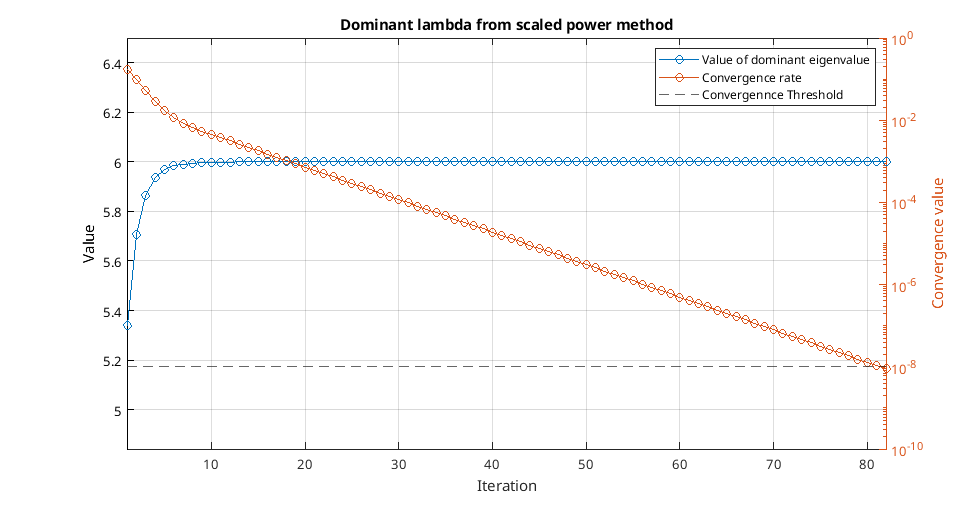
\includegraphics[width=1\textwidth]{problems/Figures/Problem2ScaledPowerMethod.png}
    \caption{Eigenvalue approximation and convergence rate over each iteration of power method.}
    \label{fig:Power}
\end{figure}

\begin{figure}[H]
    \centering
    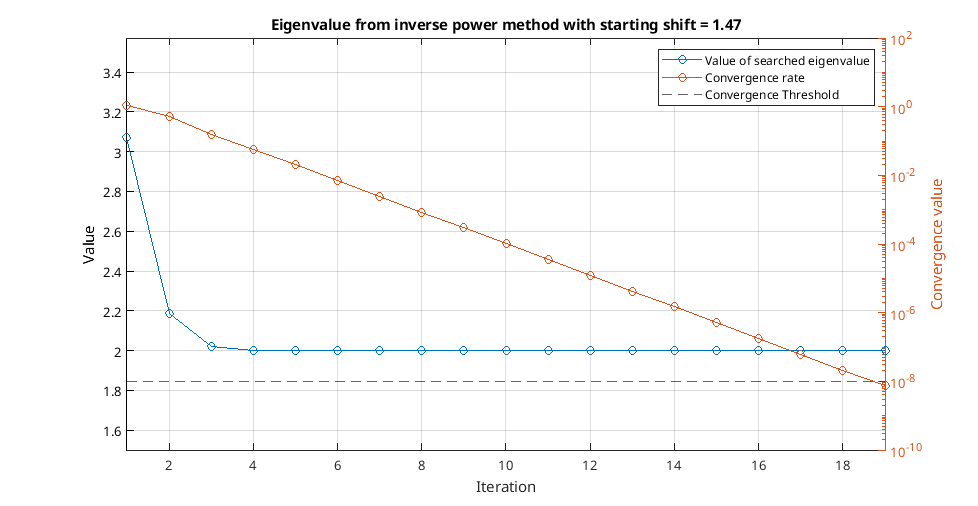
\includegraphics[width=1\textwidth]{problems/Figures/Problem2InversePowerMethod.png}
    \caption{Eigenvalue approximation and convergence rate over each iteration of inverse power method.}
    \label{fig:Inverse}
\end{figure}
% https://tobydriscoll.net/fnc-julia/krylov/inviter.html
% https://www.netlib.org/utk/people/JackDongarra/etemplates/node96.html


% Problem 3 - generate five signals with no. of samples ~1000 (maybe ~100).


%%%%%%%%%%%%%%%%%%%
%% BIBLIOGRAPHY %%%
%%%%%%%%%%%%%%%%%%%

\clearpage

\nocite{Zdunek, GoluVanl96}
\bibliographystyle{alpha}
\bibliography{bibliography}

\end{document}
